\section{Resolución}

La primera tarea realizada para la resolución fue definir las direcciones que iban a ser utilizadas.\\

En el enunciado, se especifica que del proveedor se está conectado a la subred \texttt{198.235.150.128/25}, por lo tanto, se tienen 7 bits para hosts (127 posibles) y la máscara es \texttt{255.255.255.128 = 255.255.255.10000000}. La dirección asignada al router es \texttt{198.235.150.136} con \textit{Default Gateway} \texttt{198.235.150.129}.\\

Sería un error confundir la dirección asignada al router con el Default Gateway ya que esta última es la conexión hacia el proveedor y si se pone esta conexión hacia el lado del router cuando se quiera enviar un paquete de salida habría que hacer una tabla de ruteo por cada dirección de salida que se quiere tener.\\

Del lado interno se provee la subred de clase C \texttt{198.235.151.0/24}, por lo tanto, se tienen 8 bits para hosts (255 posibles) y la máscara es \texttt{255.255.255.0 = 255.255.255.00000000}. La dirección asignada al router es \texttt{198.235.151.1}.\\

Asimismo, del lado interno se tienen 5 dependencias:
\begin{itemize}
    \item \textbf{Producción} que requiere 32 hosts por lo tanto requiere 5 bits y la máscara es /27, es decir \texttt{255.255.255.224}.
    \item \textbf{Administración} que requiere 32 hosts, es igual a producción.
    \item \textbf{Gerencia} que requiere 16 hosts por lo tanto requiere 4 bits y la máscara es /28, es decir \texttt{255.255.255.240}.
    \item \textbf{Expedición} que requiere 16 hosts, es igual que gerencia.
    \item \textbf{Comedor} que requiere 64 hosts por lo tanto requiere 6 bits y la máscara es /26, es decir \texttt{255.255.255.192}.
\end{itemize}

En el edificio 1 se tiene producción y expedición lo cual significa que se necesitan 48 hosts, por lo tanto, se requieren 6 bits y la máscara es /26, es decir \texttt{255.255.255.192} (quedan 16 direcciones IP libres).\\

En el edificio 2 en cambio se encuentran gerencia, administración y comedor lo cual significa que se necesitan 112 hosts, por lo tanto, se requieren 7 bits y la máscara es /25, es decir \texttt{255.255.255.128} (quedan 16 direcciones IP libres).\\

El enunciado también dice que la red que conecta ambos edificios tiene que ser de la mínima cantidad posible por lo tanto es una máscara /30, es decir \texttt{255.255.255.252}. Esto es porque se necesita una dirección para cada router, una para la dirección de \textit{broadcast} y otra para la dirección de red. \\

Luego, se calculan las subredes utilizadas. La dirección de red es \texttt{192.235.151.00000000} por lo tanto a continuación se proceden a especificar las subredes a utilizar para el edificio 1, 2 y la red de interconexión.\\

\begin{itemize}
    \item \textbf{Subred Edificio 1}: \texttt{198.235.151.10000000} 
    \begin{itemize}
        \item \textbf{Producción}: \texttt{198.235.151.110|00000}, la dirección IP es \texttt{198.235.151.192/27}.
        \item \textbf{Expedición}: \texttt{198.235.151.1000|0000}, la dirección IP es \texttt{198.235.151.128/28}.
    \end{itemize}
    \item \textbf{Subred Edificio 2}: \texttt{198.235.151.00000000} 
    \begin{itemize}
        \item \textbf{Administración}: \texttt{198.235.151.000|00000}, la dirección IP es \texttt{198.235.151.0/27}.
        \item \textbf{Gerencia}: \texttt{198.235.151.0010|0000}, la dirección IP es \texttt{198.235.151.32/28}.
        \item \textbf{Comedor}: \texttt{198.235.151.01|000000}, la dirección IP es \texttt{198.235.151.64/26}.
    \end{itemize}
\end{itemize}

Como el edificio 1 tiene menos conexiones IP asignadas se utilizará este mismo para la red de interconexión. Esta es \texttt{198.235.151.101000|00}, la dirección IP es \texttt{198.235.151.160/30}.\\

Por último, para verificar que ninguna red esta dentro de otra, se verifica el rango de direcciones posible (es decir la dirección máxima y mínima que puede tener un host). Se resume esta información en el siguiente cuadro:\\


\begin{table}[H]
    \rowcolors{2}{white}{lightgray}
    \centering
    \begin{tabular}{c|c|c|c}
        %\hline
        \textbf{Nombre} & \textbf{Dirección de subred} & \textbf{Dirección mínima} & \textbf{Dirección máxima} \\
        \hline
        Producción & \small\texttt{198.235.151.192/27} & \small\texttt{198.235.151.193} & \small\texttt{198.235.151.223} \\ 
        Expedición & \small\texttt{198.235.151.128/28} & \small\texttt{198.235.151.129} & \small\texttt{198.235.151.143} \\ 
        Administración & \small\texttt{198.235.151.0/27} & \small\texttt{198.235.151.1} & \small\texttt{198.235.151.31} \\ 
        Gerencia & \small\texttt{198.235.151.32/28} & \small\texttt{198.235.151.33} & \small\texttt{198.235.151.47} \\ 
        Comedor & \small\texttt{198.235.151.64/26} & \small\texttt{198.235.151.65} & \small\texttt{198.235.151.127} \\ 
        Red de interconexión & \small\texttt{198.235.151.160/30} & \small\texttt{198.235.151.161} & \small\texttt{198.235.151.162} \\ 
    \end{tabular}
    \caption{Direcciones mínimas y máximas de cada subred\\}
    \label{tabla_minmax}
\end{table}

Una vez establecidas las subredes, se procede a simular la red completa en el \textit{CORE}.

\begin{figure}[H]
    \centering
    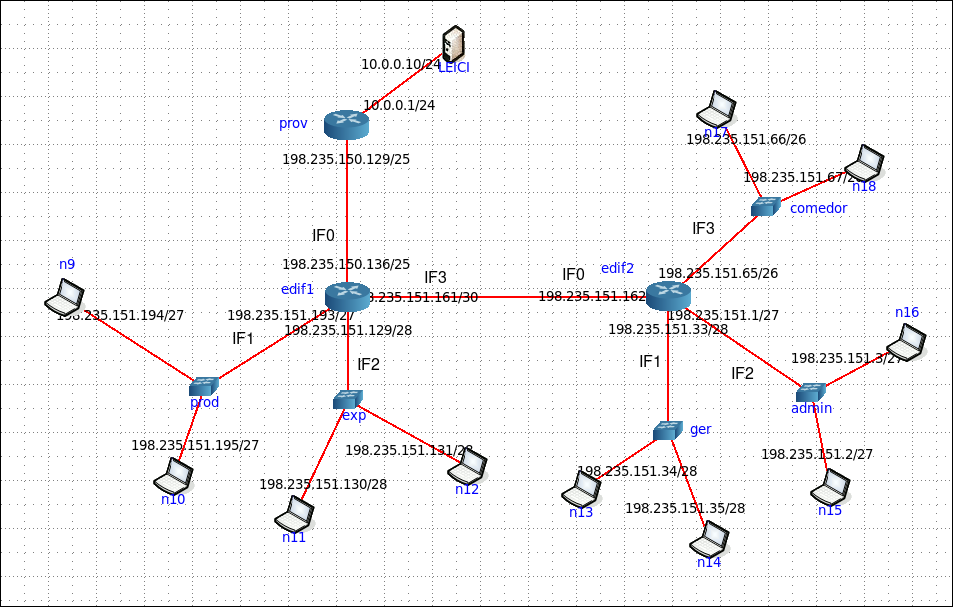
\includegraphics[scale=0.55]{Imagenes/Red.png}
    \caption{Red completa implementada en el \textit{CORE}.}
    \label{diagrama1}
\end{figure}

 Si bien las conexiones \enquote{físicas} están establecidas, deben setearse las tablas de ruteo para asegurar la comunicación entre los distintos hosts. El router del edificio 1 debe derivar las requests hacia las redes de gerencia, administración o comedor al router del edificio 2, y por default a la red del proveedor, y el router del edificio 2 debe derivar todas las request por default al router del edificio 1. Se presentan a continuación ambas tablas:\\

\begin{table}[H]
    \rowcolors{2}{white}{lightgray}
    \centering
    \begin{tabular}{c|c|c}
        \textbf{Destino} & \textbf{Dirección de destino} & \textbf{Dirección de gateway} \\
        \hline
        \small Administración & \small\texttt{198.235.151.0} & \small\texttt{198.235.150.162} \\ 
        \small Gerencia & \small\texttt{198.235.151.32} & \small\texttt{198.235.150.162} \\ 
        \small Comedor & \small\texttt{198.235.151.64} & \small\texttt{198.235.150.162} \\
        \small Expedición & \small\texttt{198.235.151.128} & \small\texttt{0.0.0.0} \\
        \small Red de interconexión & \small\texttt{198.235.151.160} & \small\texttt{0.0.0.0} \\
        \small Producción & \small\texttt{198.235.151.192} & \small\texttt{0.0.0.0} \\
        \small Proveedor & \small\texttt{198.235.150.128} & \small\texttt{0.0.0.0} \\
        \small Otro & \small\texttt{0.0.0.0} & \small\texttt{198.235.150.129} \\  
    \end{tabular}
    \caption{Tabla de ruteo del edificio 1\\}
    \label{tabla_edif1}
\end{table}

\begin{table}[H]
    \rowcolors{2}{white}{lightgray}
    \centering
    \begin{tabular}{c|c|c}
        \textbf{Destino} & \textbf{Dirección de destino} & \textbf{Dirección de gateway} \\
        \hline 
        \small Administración & \small\texttt{198.235.151.0} & \small\texttt{0.0.0.0} \\ 
        \small Gerencia & \small\texttt{198.235.151.32} & \small\texttt{0.0.0.0} \\ 
        \small Comedor & \small\texttt{198.235.151.64} & \small\texttt{0.0.0.0} \\  
        \small Red de interconexión & \small\texttt{198.235.151.160} & \small\texttt{0.0.0.0} \\
        \small Otro & \small\texttt{0.0.0.0} & \small\texttt{198.235.150.161} \\
    \end{tabular}
    \caption{Tabla de ruteo del edificio 2\\}
    \label{tabla_edif2}
\end{table}

El efecto de no tener configuradas las tablas de ruteo correctamente puede verse utilizando \textit{Wireshark}, un programa que permite capturar los paquetes que se envían por las distintas interfaces de un router. Observando, por ejemplo, la interfaz IF1 del edificio 1 (\textit{eth1}), y utilizando el terminal de un host conectado a esa boca del router (en este caso, el host n9 en 198.235.151.194) para hacer un ping al host n15 (198.235.151.2), al no tener respuesta el router contesta con \enquote{Destination unreachable}.

\begin{figure}[H]
    \centering
    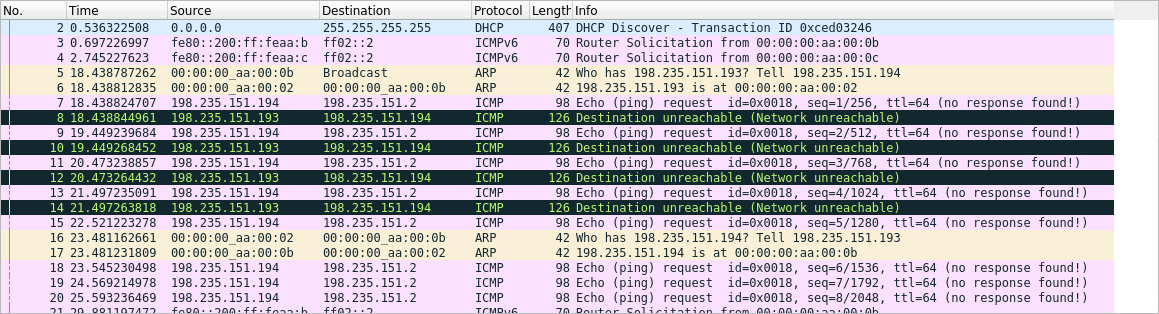
\includegraphics[scale=0.5]{Imagenes/Wireshark - Sin ruteo.png}
    \caption{Paquetes interceptados en la interfaz 1 del edificio 1 en \textit{Wireshark}. Sin tablas de ruteo.}
    \label{diagrama2}
\end{figure}

En la figura \ref{diagrama2} puede observarse además el funcionamiento del ARP, o Address Resolution Protocol, donde inicialmente el host hace un broadcast preguntando dentro de la subred, a quien corresponde el IP de la puerta de enlace, que en este caso es el router.